\chapter{Teorema de \emph{Noether}. Buscando simetrías}

	
\begin{tikzpicture}
	\fill [left color=red!50, right color=teal!50] (0,0) rectangle (6.5,.1);
	\fill [left color=teal!50, right color=blue!50] (6.5,0) rectangle (11.5,.1);
	\end{tikzpicture}

\vspace{10mm}
\begin{adjustwidth}{50pt}{50pt}
\begin{ejemplo}

%$\,$

Veremos que es lo que ocurre cuando $L=L(t)$ y, también, qué hacer si dado el $L$ no sabemos si hay o no simetría, si hay alguna forma de calcularla.

%$\,$

\end{ejemplo}
\end{adjustwidth}
\vspace{5mm}

\begin{myalertblock}{Teorema de Noether en 1 dimensión (ec \ref{T15ThNoether1-dim})}
	\begin{equation}
	\label{T17TN1d}
	\varepsilon \ \dv{K}{t} \ = \ (\var t)_S \ \pdv{L}{t} \ + \ \dv{t} \ \left[ \pdv{L}{\dot x} \ (\var x)_S \right]	
	\end{equation}
	
	\begin{equation}
		\text{Si } \ \ L\neq L(t) \quad \Rightarrow \quad Q \ = \ \pdv{L}{\dot x} \ \phi \ - \ K \, ; \quad \phi \ = \ \dfrac{(\var x)_S}{\varepsilon}
  	\end{equation}

\end{myalertblock}


\section{Reformulación del teorema de \emph{Noether}}

\begin{example}
	
\begin{equation}
\label{T16Lej1}
\text{Supongamos que nos dan el siguiente lagrangiano } L=L(t)\, : \quad \boldsymbol{ L \ = \ e^{\lambda \ t} \ m \ \dfrac {\dot x^2}{2}	} \qquad
\end{equation}
\end{example}

Para este lagrangiano no sabemos si hay o no una simetría y se puede intentar averiguarlo usando el enunciado del teorema de Noether en 1-d. Otra alternativa consiste en manipular la ecuación \ref{T17TN1d} para hacerla más vistosa: \textbf{Reformulación del teorema de Noether}.


Vimos en las ecuaciones de Hamilton (ec. \ref{T13eccHamilton}) que $\displaystyle \-\pdv{L}{t}=\dv{H}{t}$, por lo que el Th. Noether 1.d queda como:

$\displaystyle \varepsilon \dv{K}{t}=-(\var t)_S \dv{H}{t}+\dv{t} \left[\pdv{L}{\dot x} (\var x)_S \right]\, , \ $ teniendo en cuenta la derivada del producto,

$-(\var t)_S \displaystyle \dv{H}{t}=-\left\{ \dv{t}\left[ H(\var t)_S \right] - H \dv{t} (\var t)_S \right\}\, , \ $ sustituyendo arriba,

$\displaystyle \varepsilon \dv{K}{t} =  -\left\{ \dv{t}\left[ H \ (\var t)_S \right] - H \dv{t} (\var t)_S \right\} + \dv{t} \left[ \pdv{L}{\dot x} \  (\var x)_S \right]$

$\displaystyle \varepsilon \dv{K}{t} = H \dv{t} \ (\var t)_S + \dv{t} \left[ \pdv{L}{\dot x} \ (\var x)_S - H\ (\var t)_S \right] $

\begin{equation}
\label{T17TNReform1}
\displaystyle \varepsilon \dv{K}{t} - H \dv{t} \ (\var t)_S \ = \  \dv{t} \left[ \pdv{L}{\dot x} \ (\var x)_S - H\ (\var t)_S \right]	
\end{equation}

\vspace{3mm}
 Supongamos que tenemos mucha \textbf{\emph{SUERTE}}, entonces, probablemente la simetría (si la hay) sea tal que: 
 
 \begin{equation}
 \label{T17Suerte}
  \boldsymbol{\varepsilon \ \dv{K}{t} \ - \ H \ \dv{t}(\var t)_S \ = \ 0}	
 \end{equation}

En estas condiciones, automáticamente hay una cantidad conservada que ahora será

 \begin{equation}
 \label{T17SuerteQ}
  \boldsymbol{Q \ = \ \left[ \pdv{L}{\dot x} \ (\var x)_S - H\ (\var t)_S \right]}	
 \end{equation} 
 
 \vspace{3mm} Veamos que significa esto de tener  \textbf{\emph{SUERTE}}, ecuación \ref{T17Suerte}, \textcolor{gris}{$\qquad \displaystyle   \left( \varepsilon \dv{K}{t}  -  H  \dv{t}(\var t)_S  =  0 \right)$}
 
 Recordemos que $\displaystyle \ \dv{K}{t} \ $ viene del $ \ (\var L)_S \ $ lo cual implica que $\ \displaystyle (\var L)_S=\var x \pdv{L}{x} + \var t \pdv{L}{t} + \var \dot x \pdv{L}{\dot x} =\varepsilon \dv{K}{t}\, , \ $ 
 
 por lo que la ecuación ecuación \ref{T17Suerte} será: $\ \displaystyle (\var x)_S \pdv{L}{x} + (\var t)_S \pdv{L}{t} + (\var \dot x)_S \pdv{L}{\dot x}- H \dv{t} \ (\var t)_S=0$
 
 Recordando la definición de Hamiltoniano en  1-d, ec \ref{T13inicio},  $\ \displaystyle H=\pdv{L}{\dot x} \dot x - L$
 
$\ \displaystyle (\var x)_S \ \pdv{L}{x} \ + \ (\var t)_S \ \pdv{L}{t} \ + \ 
(\var \dot x)_S \ \pdv{L}{\dot x} \ - \left( \pdv{L}{\dot x} \dot x - L \right) \ \dv{t} \ (\var  t)_S=0 , , \ $ sacando $(\var \dot x)_S$ factor común,

\begin{equation}
\label{T17Suerte2}
\boldsymbol{
(\var x)_S\ \pdv{L}{x} \ + \ (\var t)_S\ \pdv{L}{t} +
\textcolor{red}{\left( (\var \dot x)_S \ - \ \dot x \ \dv{t} \ (\var t)_S \right)} \ \pdv{L}{\dot x}
 \ + \ L\ \dv{t} \ (\var t)_S \ = \ 0
}	
\end{equation}

\vspace{3mm}
\begin{ejemplo}
\underline{Atención}: Ala expresión	 $\ \displaystyle \textcolor{red}{\left( (\var \dot x)_S \ - \ \dot x \ \dv{t} \ (\var t)_S \right)} \ $ muchos autores le llaman simplemente $\ \textcolor{blue}{\ \var \dot x \ } \ $ es solo cuestión de definición y en este curso no se va utilizar esa notación. Para nosotros, $\displaystyle \var \dot x=\dv{t} (\var x)$.
\end{ejemplo}
\vspace{5mm}


Pues bien, el factor \textbf{\emph{SUERTE}} va a querer decir que si somos capaces de encontrar $\ (\var x)_S,\ (\var t)_S,\ (\var \dot x)_S$ que cumplan la relación \ref{T17Suerte2}, que parece una monstruosidad pero luego veremos que no es para tanto al aplicarlo al ejemplo 17.1. La \textbf{\emph{recompensa}} es que tendremos de inmediato la cantidad conservada, ec \ref{T17SuerteQ}.

\vspace{5mm}
El teorema de Noether reformulado queda como:

\begin{large}
\begin{myblock}{Teorema de Noether 1-d reformulado}
$\ $
\begin{equation} \label{T17TNReformulado}
\begin{split}
\subrayado{\ \boldsymbol{ (\var x)_S\ \pdv{L}{x} \ + \ (\var t)_S\ \pdv{L}{t} +
\left( (\var \dot x)_S \ - \ \dot x \ \dv{t} \ (\var t)_S \right) \ \pdv{L}{\dot x}
 \ + \ L\ \dv{t} \ (\var t)_S \ = } \ }\\ 
\subrayado{ \ \boldsymbol{ = \ \dv{t} \ \left[ \pdv{L}{\dot x} \ (\var x)_S \ - \ H\ (\var t)_S \right]} \ }	
\end{split} 
\end{equation}
$\ $
\end{myblock}
\end{large}

\vspace{5mm}

\begin{ejemplo}
$^*$ Si probásemos este método con el lagrangianao del ejemplo introductorio del tema \ref{NoeterIdeII} (Teorema de Noether I/II), $\ L=m\dfrac{\dot x^2}{2}-\dfrac{a}{x^2}\ $ no tendríamos \emph{SUERTE}, el primer miembro del teorema de Noether reformulado no sería cero y $Q$ no sería una cantidad conservada. El teorema completo sí se verificaría, por supuesto, pero no daría cero, no habría \emph{suerte}, no habría cantidad $Q$ conservada.
\end{ejemplo}


\vspace{10mm}

\begin{adjustwidth}{20pt}{20pt}
\begin{destacado}
\textbf{?`Cómo saber si usar el teorema de Noether, \ref{T17TN1d}, o el teorema de Noether reformulado \ref{T17TNReformulado}?}

La respuesta es sencilla: si $L\neq L(t) \ \Rightarrow \ $ teorema de Noether, \ref{T17TN1d}; si $L=L(t) \ \Rightarrow \ $ suele ser mejor teorema de Noether reformulado \ref{T17TNReformulado}.
\end{destacado}
\end{adjustwidth}

\vspace{10mm}

\section{Búsqueda de la simetría}

Nuestro objetivo es saber cual es la simetría (si es que la hay), $\ (\var x)_S,\ (\var y)_S,\ (\var z)_S \,  \   $ y ojalá que tengamos \emph{SUERTE}, podría ocurrir que hubiese simetría y no tuviésemos suerte (comentario anterior $^*$).

Las transformaciones infinitesimales tienen la forma:

$$ \boldsymbol{ (\var x)_S \ = \ \varepsilon \ f(x,t) \, ; \qquad (\var t)_S \ = \ 	\varepsilon \ g(x,t) }$$

De ahí, $\quad \displaystyle \boldsymbol{(\var \dot x)_S}=\varepsilon \dot f =\varepsilon \left( \pdv{f}{x} \dot x + \pdv{f}{t} \right) = \boldsymbol{\varepsilon (f_x \dot x , f_t)}\, , \ $ usando la notación $\ \displaystyle f_x=\pdv{x}{x} \text{ y } f_t=\pdv{f}{t}$.

Recordemos nuestro lagrangiano, $\ L=e^{\lambda t} m \dfrac{\dot x^2}{2} \, , \  $ calculemos las derivadas parciales necesarias y calculemos el primer miembro de la ecuación del teorema de Noether reformulado \ref{T17TNReformulado}

\vspace{4mm}
$\triangleright\ $ Primer término:

\begin{adjustwidth}{20pt}{20pt}
	$\displaystyle \pdv{L}{x}=0 \ \to \ (\var x)_S \pdv{L}{x}=0$
\end{adjustwidth}

\vspace{4mm}
$\triangleright\ $ Segundo término:

\begin{adjustwidth}{20pt}{20pt}
	$\displaystyle \pdv{L}{t}=\lambda \ e^{\lambda t} m \dfrac{\dot x^2}{2} \ \to \ (\var t)_S \pdv{L}{t}=\varepsilon \ g \ \lambda \ e^{\lambda t} m \dfrac{\dot x^2}{2}$
\end{adjustwidth}

\vspace{4mm}
$\triangleright\ $ Tercer término: 

\begin{adjustwidth}{20pt}{20pt}
	$\displaystyle (\var \dot x)_S - \dot x\dv{t} (\var t)_S = \varepsilon (f_x \dot x+f_t) - \dot x\dv{t}(\varepsilon g)= 
	\varepsilon (f_x \dot x+f_t) - \dot x \varepsilon (g_x \dot x+g_t)=
	\varepsilon [f_x \dot x -f_t-g_x \dot x^2 -\dot x g_t]=
	\varepsilon[(f_x-g_t)\dot x-g_x\dot x^2+f_t] \ \to \ \left( (\var \dot x)_S - \dot x\dv{t} (\var t)_S \right)  \pdv{L}{\dot x}=
	\varepsilon[(f_x-g_t)\dot x-g_x\dot x^2+f_t] \ e^{\lambda t} m \dot x = \varepsilon [(f_x-g_t)\dot x^2-g_x \dot x^3+f_t \dot x] e^{\lambda t} m $
\end{adjustwidth}

\vspace{4mm}
$\triangleright\ $ Cuarto término:

\begin{adjustwidth}{20pt}{20pt}
	$\displaystyle L\dv{t} (\var t)_S = \varepsilon \dot g L =\varepsilon \dot g e^{\lambda t} m \dfrac{\dot x^2}{2}$
\end{adjustwidth}
\vspace{4mm}

 Con todo esto, nos preguntamos si el primer miembro de la ecuación del teorema de Noether reformulado \ref{T17TNReformulado} será cero:
 $\quad \displaystyle \varepsilon \left \{ g \lambda e^{\lambda t} m \dfrac{\dot x^2}{2} + \left[ (f_x-g_t)\dot x^2 -g_x \dot x^3 + f_t \dot x \right] e^{\lambda t} m+ \dot e e^{\lambda t} m \dfrac{\dot x^2}{2} \right\} \ \begin{matrix} \textbf{?} \\ = \\  \\ \end{matrix} \ 0$
 
 \vspace{4mm}
 Para cada curva $x(t)$ que sustituyamos tendremos una ecuación distinta, parece que tenemos infinitos grados de libertad. ?`Cómo podremos asegurar que esto sea cero para cualquier curva $x(t)$ que nos inventemos?
 
 Escribamos esta última expresión agrupando en potencias de $\dot x$,
 
 $\displaystyle \dot x \ [2f_t] \ + \ \dot x^2 \ [g \lambda + 2(f_x-g_t) + \dot g] \ + \ \dot x^3 \ [-2g_x] \ \begin{matrix} \textbf{?} \\ = \\  \\ \end{matrix} \ 0$
 
 Para poder asegurar que esto sea cero para cualquier curva $x(t)$, es necesario que los coeficientes de las potencias de $\dot x$ sean todos cero.
 
 $\begin{cases}
\ \ \ 2f_t=0 \ \to \ \displaystyle \pdv{f}{t}=0 \ \to \ f=f(x) \\
\ - 2g_x=0 \ \to \ \displaystyle	 \pdv{g}{x}=0 \ \to \ g=g(t) \\
\ \ \ g\lambda + 2(f_x-g_t)+	\dot g=0
\end{cases} \to \text{ Transf. infinitesimal } \
\begin{cases}
\ \ (\var x)_S & \ = \ \varepsilon \ f(x) \\
\ \ (\var t)_S & \ = \ \varepsilon \ g(t) \\
\ \ (\var \dot x)_S & \ = \ \varepsilon \ (f_x \dot x + f_t)
\end{cases}$

La tercera ecuación anterior, que provenía de hacer cero el coeficiente en $\dot x^2$, la podemos escribir como  $\ g \lambda + 2 f'(x)-2g'(t)+g'(t)=0$, es decir, tenemos la ecuación diferencial $\ g\lambda+ 2 f'(x)-g'(t)=0\, , \ $ que, en principio, puede parecer muy complicada pero realmente no lo es:
$\ g'(t)-\lambda g(t)=2f'(x)$ es una EDO de variables separables, $F'(x)=G'(t)$, cuya única solución posibles es que $F(x)=G(t)=cte=K$, así:

$\begin{cases}
\ 2f'(x)=K \ \to \ 	\boldsymbol{\boxed{\  f(x)=\dfrac k 2 x \ }} \\
\ g'(t)-\lambda g(t)=K  \ \to \ \begin{matrix} \text{EDO} \\ \text{1-orden} \end{matrix} \ \to  \ \displaystyle \dv{g}{t}=K+\lambda g \to \dfrac 1 \lambda \int
 \dfrac{\lambda \ \dd t}{k+\lambda g}=\int \dd t \to \boldsymbol{ \ g(t)=\dfrac{B e^{\lambda t}-k}{\lambda}}
 \end{cases}$
 
\begin{footnotesize}\textcolor{gris}{
$\displaystyle  \left( 
 \dfrac 1 \lambda \int \dfrac{\lambda \ \dd t}{k+\lambda g}=\int \dd t  \to  \dfrac 1 \lambda \ \ln (K+\lambda g)=t + A \to   \ln (K+\lambda g)=t \lambda + A \lambda  \to k+\lambda g =e^{\lambda t} e^{\lambda A}=B e^{\lambda t}\ \to \
	g(t)=\dfrac{B e^{\lambda t}-k}{\lambda} \right)$
} \end{footnotesize}

Una familia de soluciones para $g$ es $\quad \boldsymbol{ \boxed{ \ g(t) \ }} \ = \dfrac B \lambda e^{\lambda t} = \ \boldsymbol{\boxed{\ Ce^{\lambda t} - \dfrac k \lambda \ }}$
 
 
Con todo ello, tenemos que $\ (\var t)_S=\varepsilon \left( Ce^{\lambda t} - \dfrac k \lambda \right)\, , \  $ por lo que $\ t'=t+\varepsilon \left( Ce^{\lambda t} - \dfrac k \lambda \right)\, $ que es nuestra transformación infinitesimal para $t$.

Si $\ t>>1 \ \to \ Ce^{\lambda t} >>1 \ \to \ $ imponemos $\boldsymbol{ \ C =0 \,  } , \ $ con lo que $\ t'\approx t- \varepsilon \dfrac k \lambda \ \to \ \boldsymbol{(\var t)_S=-\varepsilon \dfrac k \lambda}$

Ya tenemos nuestras variaciones infinitesimales de la simetría, $\ \boldsymbol{ (\var x)_S=\varepsilon \dfrac k 2 x  }\  \text{ y }\ \boldsymbol{(\var t)_S = -\varepsilon \dfrac k \lambda} \, . \ $ Hemos tenido \emph{SUERTE}, el primer miembro de la ecuación del teorema de Noether reformulado es cero, luego hay una cantidad $\ Q=\displaystyle \pdv{L}{\dot x} (\var x)_S - H(\var t)_S = cte$, particularizando (eliminamos los $\varepsilon$ por sencillez),

$Q=\displaystyle \pdv{L}{\dot x} (\var x)_S - H (\var t)_S=e^{\lambda t} m \dot x \dfrac k 2 x + H \dfrac k \lambda\, , \ $ como $\ H=\displaystyle \pdv{L}{	\dot x} \dot x - L=e^{\lambda t} m \dot x \dot x - e^{\lambda t}\dfrac m 2 \dot x=  \dfrac 1 2 e^{\lambda t} m \dot x^2 \, , \ $ 

sustituyendo en $Q\, , \qquad \tilde{Q}=\dfrac Q k = cte = e^{\lambda r} \dfrac m 2 [\dot x x + \dfrac{\dot x^2}{\lambda}] \ \to \ $ multiplicando por $\ \lambda=cte\, , $

$\tilde{\tilde Q}=cte=e^{\lambda t} \dfrac m 2 [\lambda \dot x x+ \dot x^2]$. Comprobemos que es constante:


$\displaystyle \dot{\tilde{\tilde Q}}=\dfrac m 2 [\lambda e^{\lambda t} (\lambda \dot x x+\dot x^2) +e^{\lambda t} (\lambda \ddot x x + \lambda \dot x^2 + 2 \dot x \ddot x ] =
	\dfrac m 2 e^{\lambda t} [ \lambda^2 \dot x x 
	+\lambda \dot x^2 + \lambda \ddot x x + \lambda \dot x^2 + 2 \dot x \ddot x ]$
	
	$\displaystyle \dot{\tilde{\tilde Q}}= 
	\dfrac m 2 e^{\lambda t} [ 2\lambda \dot x^2 + \lambda^2 \dot x x +(\lambda x + 2\dot x) \ddot x ] \, . \ $
 Veamos las ecuaciones E-L del movimiento:
 
 $\displaystyle \dv{t}\pdv{L}{\dot x}=\pdv{L}{x} \ \to \ \dv{t} \left( e^{\lambda t} m \dot x º\right) = 0 \ \to \ \lambda e^{\lambda t} m \dot x + e^{\lambda t} m \ddot x = 0 \ \to \ \lambda \dot x + \ddot x =0 \ \to \ \boldsymbol{\ddot x=-\lambda \dot x} $ 
 
 Sustituyendo $\quad \displaystyle \dot{\tilde{\tilde Q}}= 
 \dfrac m 2 e^{\lambda t} [ 2\lambda \dot x^2 + \lambda^2 \dot x x + (\lambda x+2\dot x) (-\lambda \dot x) ] = 
 \dfrac m 2 e^{\lambda t} [\bcancel{ 2\lambda \dot x^2 }+ \cancel{\lambda^2 \dot x x } - \cancel{\lambda^2 \dot x x} - \bcancel{2\lambda \dot x^2} ]=0  $
 
Efectivamente, hay una cantidad conservada a lo largo de la trayectoria de la partícula.

\vspace{10mm}

\begin{adjustwidth}{25pt}{25pt}
\begin{destacado}
Recapitulando:

$\qquad$ Para $\quad L \ = \ e^{\lambda t} \ m \ \dfrac{\dot x^2}{2}$

$\qquad$ La cantidad conservada es $\quad Q \ = \ e^{\lambda t} \ \dfrac m 2 \ (\lambda \dot x x + \dot x^2 ) \ = \ cte$

$\qquad$ Debido a la simetría $\quad \begin{cases} \ (\var x)_S \ = \ \varepsilon \ \dfrac x 2 \ \lambda \\ \ (\var t)_S \ = \ - \varepsilon  \end{cases}$	
\end{destacado}	
\end{adjustwidth}

\begin{small}
Por simplificar, como $k=cte$ cualquiera, hemos tomado $k=\lambda$ y, entonces,  $\ \begin{cases} \ (\var x)_S=\varepsilon \dfrac k 2 x = \varepsilon \dfrac \lambda 2 x \\ \ (\var t)_S=-\varepsilon \dfrac k \lambda = -\varepsilon \dfrac \lambda\lambda = -\varepsilon  \end{cases}$
\end{small}
	
\vspace{5mm}

\begin{ejemplo}
Como $L=L(t) \to H\neq cte$ \textcolor{gris}{$\left(\dv{H}{t}=-\pdv{L}{t} \right)$}. Nuestro lagrangiano solo es cinético, $L=e^{\lambda t} \frac m 2 \dot x^2=T$, cuando hemos calculado $H$ ha coincidido con $T$, por lo que $H=L=T=E$, pero no es constante. Hasta ahora, en todos los casos que hemos visto ocurría que $E=H=cte$, ahora ya tenemos un caso en que esto no ocurre.
\end{ejemplo}


\vspace{5mm} Nuestra transformación infinitesimal de simetría es $(\var x)_S=\varepsilon \dfrac \lambda 2 x \ \text{ y } \ (\var t)_S=-\varepsilon$, pero \textbf{?`cuál es la transformación de simetría finita?} \textcolor{gris}{En el capítulo \ref{NoeterIdeII} vimos que la transformación de simetría $x\to \lambda x \ \text{ y } \ t\to \lambda^2 t$ daba lugar a la transformación infinitesimal $(\var x)_S=\varepsilon (x-2\dot x t) \ \text{ y } \ (\var t)_S=\varepsilon 2 t$} 

Buscar la transformación finita de simetría asociada a una transformación inifinitesimal dada se puede hacer de varios modos, vamos a ver dos de ellos: \emph{A) método de las congruencias finitas} y  \emph{B) método de entender qué es lo que está pasando}.

\vspace{5mm}
\subsection{Búsqueda de la transformación finita de simetría conociendo la transformación infinitesimal}
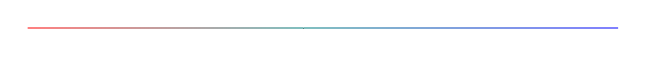
\begin{tikzpicture}
	\fill [left color=red!50, right color=teal!50] (0,0) rectangle (3.5,.01);
	\fill [left color=teal!50, right color=blue!50] (3.5,0) rectangle (7.5,.01);
	\end{tikzpicture}
\vspace{5mm}

------ \emph{A) método de las congruencias finitas} 

\begin{adjustwidth}{20pt}{20pt}

	\begin{multicols}{2}
	\begin{figure}[H]
	\centering
	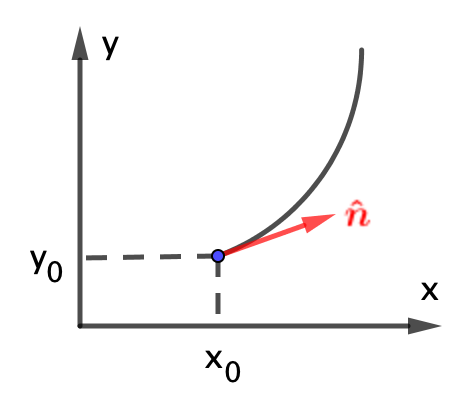
\includegraphics[width=.3\textwidth]{imagenes/img17-01.png}
	\end{figure}
	$(\var x)_S=\varepsilon \dfrac \lambda 2 x \ \text{ y } \ (\var t)_S=-\varepsilon$
	
	Parametrizamos la curva de la simetría, $(t(s),x(s))$, el vector unitario tangente a la trayectoria es 
	
	$\hat n=\left( \displaystyle \dv{t}{s}, \dv{x}{s} \right)$
	\end{multicols}
	Cerca de $s=0 \to (t=0,x=0)$, si sumamos la cantidad $\varepsilon \left(-1+\dfrac x 2 \lambda \right)$ iremos a un punto infinitesimalmente cercano: $(t_0,x_0) \ \to \ (t_0,x_0)+\varepsilon \left(-1+\dfrac x 2 \lambda \right)=(t.x)$, siempre que $s<<1$. Podemos interpretar el factor $\left(-1+\dfrac x 2 \lambda \right)$ como una especie de velocidad, $x=x_0+vt$, tangente a la trayectoria, el vector $\hat n=\left(-1+\dfrac x 2 \lambda \right)$, tangente en todo momento a la trayectoria.
	Vamos a buscar la \emph{congruencia}, la curva cuyos vectores tangentes son los $\hat n$.
	
	$\displaystyle \left(\dv{t}{s}, \dv{x}{s} \right)=\left(-1+\dfrac x 2 \lambda \right) \ \to \ \begin{cases}
 		\ \displaystyle \dv{t}{s}=-1 &\to \ t=-s+A \\
 		\ \displaystyle \dv{x}{s}=\dfrac \lambda 2 x &\to x=Be^{\frac \lambda 2 s} \end{cases}$
 		
 	Para $s=0 \to (t_0,x_0) \to \begin{cases} \ t=-s+t_0 & (A=t_0) \\ \ x=x_0e^{\frac \lambda 2 s} &(B=x_0)  \end{cases}$, 
 	
 	por lo que la transformación finita de simetría es:
 	
 	$$\boldsymbol{ \boxed{ \ \begin{matrix} t' \ = \ t - s \\ x'\ = \ x e^{\frac \lambda 2 s} \end{matrix} \ } }$$	
 
\end{adjustwidth}



------ \emph{B) método de entender qué es lo que está pasando}.

\begin{adjustwidth}{20pt}{20pt}
	En un pequeño paso $\varepsilon$, pasamos de una posición $(t,x)$ a otra$(t',x')$, en dos pasos $\varepsilon$ llegaremos a $t'',x'')$, y así: 
	
	\begin{small} $\begin{cases} \ (\var t)_S=-\varepsilon \\ 	\ (\var x)_S=\varepsilon \dfrac \lambda 2 x \end{cases} \ \to \  \begin{cases} 
	 \ t'=t-\varepsilon \\ \ x'=x+ \varepsilon \dfrac \lambda 2 x \end{cases} \ \to \ 
	 \begin{cases} \  t''=t'-\varepsilon = t-2\varepsilon \\  \  x''=x'+\varepsilon \dfrac \lambda 2 x' = \left(1+\varepsilon \dfrac \lambda 2 \right) \left(x+\varepsilon \dfrac \lambda 2 x \right) =x  \left(1+\varepsilon \dfrac \lambda 2 \right)^2\end{cases}$ \end{small}
	 
	 Para llegar al punto final $(t^F,x^F)$ necesitaremos realizar $N$ de estos pasitos $\varepsilon$ y tomaremos límite cuando $N$ tienda a $\infty$. Como $N\varepsilon =s \to \varepsilon = s/N$
	 
	  $\quad \begin{cases} \ t^F=t-s\\ \ x^F=x\left(1+\dfrac s N \dfrac \lambda 2\right)^N \end{cases} \quad \to \quad \displaystyle \lim_{N\to \infty}{\left(1+\dfrac{s\lambda}{2N} \right)^N\ x } = e^{s\lambda/2} x$
	  
	\begin{footnotesize}
	\textcolor{gris}{
	$\displaystyle \lim_{N\to \infty}{\left(1+\dfrac{s\lambda}{2N} \right)^N\ x } =\lim_{N\to \infty}{\left(1+\dfrac{s\lambda/2}{N} \right)^N\ x } =e^{s\lambda/2} x\, ; \quad \text{ya que} \quad  \lim_{\Box\to \infty} \left( 1+\dfrac{algo}{\Box}\right)^{\Box} =e^{{algo}}$}	\end{footnotesize}
 	 
 	\vspace{5mm} Finalmente,  la transformación finita de simetría es:
 	
 	$$\boldsymbol{ \boxed{ \ \begin{matrix} t^F \ = \ t - s \\ x^F\ = \ x e^{\frac \lambda 2 s} \end{matrix} \ } }$$	
 
 	Que coincide, obviamente, con la encontrada con el método anterior.
 	
 	Hay otros métodos para encontrar la simetría a partir de la transformación infinitesimal, como el de los vectores de Killing.
\end{adjustwidth}

\begin{center}\rule{200pt}{0.1pt}\end{center}


\vspace{5mm} \textbf{Comprobación de que la transformación finita encontrada por  ambos métodos es realmente una simetría.}

$\begin{cases} \ t'=t-s \to t=t'+s \, ; \quad \dd t'=\dd t \\ \ x'=xe^{\lambda s/2} \end{cases}$

$s=\displaystyle \int_{t_1}^{t_2} L \dd t$, como $\dd t=\dd t'$, la acción es invariante si lo es el lagrangiano.

$L=e^{\lambda t} \dfrac m 2 \dot x^2$

$\dot x'=\displaystyle \dv{x'}{t'}=\dv{t}{t'}\dv{x'}{t}=1\cdot \dv{x'}{t}=\dot x e^{\lambda s/2} \ \to \ \dot x=e^{-\frac \lambda 2 s} \dv{x'}{t'} \ \to \ \dot x'^2=e^{-\lambda s} \displaystyle \left( \dv{x'}{t'} \right)^2 $

Luego,  $\quad L=e^{\lambda(t'+s)} \dfrac m 2 e^{-\lambda s} \displaystyle \left( \dv{x'}{t'} \right)^2=e^{\lambda t'} \dfrac m 2 \dot x'^2=L'\, , \ $ invariante.

Luego efectivamente la transformación corresponde a una simetría. \hspace{5cm}$\Box$


